\documentclass[final, hyperref, table]{beamer}
\mode<presentation>
{ 
\usetheme{TF}
 }

 \usepackage[english,francais]{babel} % "babel.sty"
% \usepackage{french}                  % "french.sty"
%  \usepackage{franglais}               % "franglais.sty" (a defaut)
  \usepackage{times}			% ajout times le 30 mai 2003
 
%% --------------------------------------------------------------
%% CODAGE DE POLICES ?
%% Si votre moteur Latex est francise, il est conseille
%% d'utiliser le codage de police T1 pour faciliter la césure,
%% si vous disposez de ces polices (DC/EC)
\usepackage[utf8]{inputenc}
\usepackage[T1]{fontenc}


%% ==============================================================
%\usepackage{graphicx}
\usepackage{amsmath,amsfonts}
%\usepackage[table]{xcolor}
\usepackage{subfigure}
\usepackage{fancybox}
%\usepackage{hyperref}
\usepackage{multicol}
\usepackage{wrapfig}
\usepackage{listings}
\usepackage{xcolor}
\usepackage[orientation=portrait,size=a0,scale=1.4]{beamerposter}

% Display a grid to help align images
%\beamertemplategridbackground[1cm]

%We will get the normal bibliography style (number or text instead of icon) by including the following code
\setbeamertemplate{bibliography item}[text]
\setbeamerfont{caption}{size=\footnotesize}
% listings settings
\definecolor{lstComments}{rgb}{0,0.6,0}
\definecolor{lstBkgrd}{rgb}{1,1,0.8}
\lstset{%
  language=Python, % the language of the code
  frame=single,  % adds a frame around the code
  commentstyle=\color{lstComments},% comment style
  backgroundcolor=\color{lstBkgrd},   % choose the background color
  basicstyle=\scriptsize,       % the size of the fonts that are used for the code
  keywordstyle=\color{blue},      % keyword style
  showstringspaces=false,          % underline spaces within strings only
}
\title[TELEMETA, open web audio platform for
sound archives]{TELEMETA : open web audio platform for
sound archives\\in the use case of
ethnomusicology}

\author[Fillon, Pellerin, Brossier, Simonnot]{Thomas Fillon \inst{1,2}, Guillaume Pellerin\inst{1}, Paul Brossier\inst{1}, Jos{\'e}phine Simonnot\inst{3}}


\institute[Parisson]{\small
  \inst{1}%
  Parisson, France\\
  \inst{2}%
  LAM, Institut Jean Le Rond d'Alembert, UPMC Univ. Paris 06, UMR CNRS 7190,
    11 rue de Lourmel, 75015 Paris, France\\
 \inst{3}%
  CREM, LESC, UMR CNRS 7186, MAE, Université Paris Ouest Nanterre La Défense,
21 Allée de l'Université - 92023 Nanterre, France\\
%Thanks
\vskip1ex
 {\small \textcolor{red}{\emph{This work was partially done inside the DIADEMS project\\ funded by the French National Research Agency ANR (CONTINT)}}}
}

\date[03/09/2013]{03 septembre 2013}
%\usebackgroundtemplate{\centering \includegraphics[width=\paperwidth]{../presentation/piano_wallpaper_red.png}}
\begin{document}
%\maketitle
\begin{frame}[containsverbatim]{}%\pgfsetfillopacity{0.9}
% ==================================
% --------- Résumé -----------------
% ==================================
  \begin{block}{Abstract}\small

    \begin{minipage}{0.74\linewidth}
      \begin{itemize}
      \item \emph{Telemeta} is an \alert{open-source audio web Content
        Management System} (CMS) dedicated to \alert{digital sound
          archives} secure storing, indexing and publishing.
      \item The demonstration presents the features of this platform
        in the context of \alert{\emph{ethnomusicological} research}.
      \item It focuses on the enhance and collaborative
        user-experience in accessing audio items and their associated
        metadata and on the possibility for the expert user to further
        enrich those metadata.
      \item \emph{Telemeta} also provides integrated \alert{audio signal
        processing tools} for automatic analysis of sound items.
      \end{itemize}
    \end{minipage}
    \begin{minipage}{0.24\linewidth}
      \begin{center}
        \includegraphics[scale=0.9]{img/logo_telemeta_1-1.pdf}
    
        \hspace{-3cm}\colorbox{yellow!50}{\Large \textbf{\url{http://telemeta.org/}}}
      \vskip1ex
      \colorbox{yellow!50}
      { Contact : \href{mailto:guillaume@parisson.com}{guillaume@parisson.com} }
     \end{center}
 \end{minipage}
 \colorbox{red!20}{\textbf{KEYWORDS : Sound archives, Metadata, Ethnomusicology, Database, Audio labelling, Web platform}}
   \end{block}
 
% ==================================
% --------- Corps -----------------
% ==================================
  \begin{columns}[t]
\footnotesize
% ==================================
% --------- Colonne gauche ---------
% ==================================
 \begin{column}[T]{.49\linewidth}
    \begin{block}{Introduction}
    \textbf{Needs}\\
      \begin{itemize}
      \item In social sciences like anthropology and linguistics,
        researchers have to work on multiple types of multimedia
        documents such as photos, videos, sound recordings or
        databases.
      \item The need to easily access, visualize and annotate
        such materials can be problematic given their diverse formats,
        sources and given their chronological nature.
      \end{itemize}

\textbf{The \emph{Telemeta} project}\\
\begin{itemize}
\item The CREM laboratory and Parisson have been developing an innovative,
  collaborative and interdisciplinary open-source web-based multimedia
  platform since 2007.
\item Goal : fit the professional requirements from both sound archivists and
  researchers in ethnomusicology.
\item Official Platform online since 2011 : \emph{Archives sonores du CNRS, Musée de
    l'Homme}: 
\end{itemize}
\begin{center}
  \colorbox{yellow!50} {\normalsize \hskip3ex \bf \url{http://archives.crem-cnrs.fr} \hskip3ex }
\end{center}

    \end{block}

\begin{block}{Web audio content management features and architecture}
  \begin{itemize}
  \item \emph{Telemeta} is a free and open source ({\scriptsize CeCILL
      Free Software License Agreement}) web audio content management
    system which introduces efficient and secure methods for
    \alert{backuping}, \alert{indexing}, \alert{transcoding}, \alert{analysing} and \alert{publishing} any
    digitalized audio file with its metadata.
  \item \emph{Telemeta} is ideal for
    professional collaborators who wants to easily organize, backup, archive and
    publish documented sound collections of audio files, CDs,
    digitalized vinyls and magnetic tapes over a strong database in
    accordance with \alert{open web standards}.
  \item \emph{Telemeta} architecture
    is \alert{flexible} and can easily be adapted to particular database
    organization of a given sound archives.
  \end{itemize}

\begin{figure}[htbp]
  \centering
  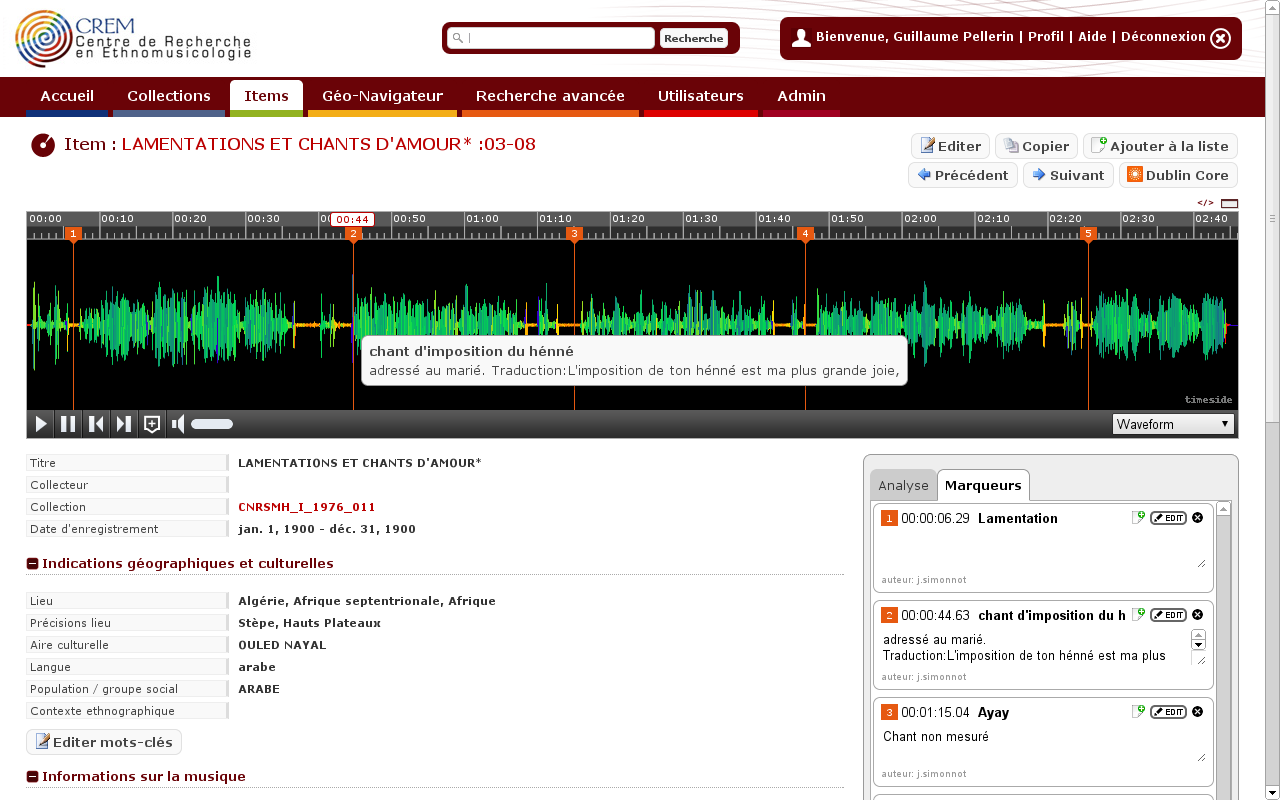
\includegraphics[width=0.47\paperwidth]{img/player_mark.png}
  \caption{Screenshot excerpt of the \emph{Telemeta} web interface}
\end{figure}



The main features of \emph{Telemeta} are:
\vspace{-0.1cm}
\begin{itemize}
\item \alert{Pure HTML} web user interface including high level \alert{search engine}
\item \alert{Smart workflow management} with contextual user lists, profiles and rights
  % \item RSS and JSON feed generators
  % \item XML serialized backup
\item Model-View-Controller (\alert{MVC}) architecture 
\item Strong Structured Query Language (\alert{SQL}) or Oracle backend

\end{itemize}
Beside database management, the audio support is mainly provided through an external component, \emph{TimeSide}.

\end{block}
\begin{block}{Metadata}
  \begin{itemize}
  \item In addition to the audio data, an efficient and \alert{dynamic
    management} of the associated metadata is also required.
  \item Dynamically handling metadata in a \alert{collaborative} manner optimises
    the continuous process of knowledge gathering and enrichment of
    the materials in the database.
  \item Interoperability : integration of the metadata standards protocols \alert{Dublin Core}
    and \alert{OAI-PMH} (Open Archives Initiative Protocol for Metadata
    Harvesting) \cite{DublinCore,OAI-PMH}.
  \end{itemize}

\textbf{Contextual Information}\\
In ethnomusicology, contextual information could be geographic, cultural and musical. It could also store archive related information and include related materials in any multimedia format. 

\textbf{Annotations and segmentation}\\
Metadata also consist in temporal information such as:
\begin{itemize}
\item a list of \alert{time-coded markers} associated with annotations
\item a list of of \alert{time-segments} associated with labels.
\end{itemize}
The ontology for those labels is relevant for ethnomusicology (e.g. speech versus singing voice segment, chorus, ...).
It should be noted that annotations and segmentation can be done either by a human expert or by some automatic signal processing analysis.

\end{block}
    \end{column}
   
% ==================================
% ------- Colonne droite -----------
% ==================================
\begin{column}[T]{.49\linewidth}
  \begin{block}{TimeSide : open web audio processing framework}
One specificity of the \emph{Telemeta} architecture is to rely on an external component, \emph{TimeSide}, that offers audio player integration together with low and high level audio signal processing capabilities.

\begin{center}
  \colorbox{yellow!50}{\bf \hskip3ex \url{https://github.com/yomguy/TimeSide/} \hskip3ex  }
\end{center}

    \begin{figure}[htbp]
  \centering
  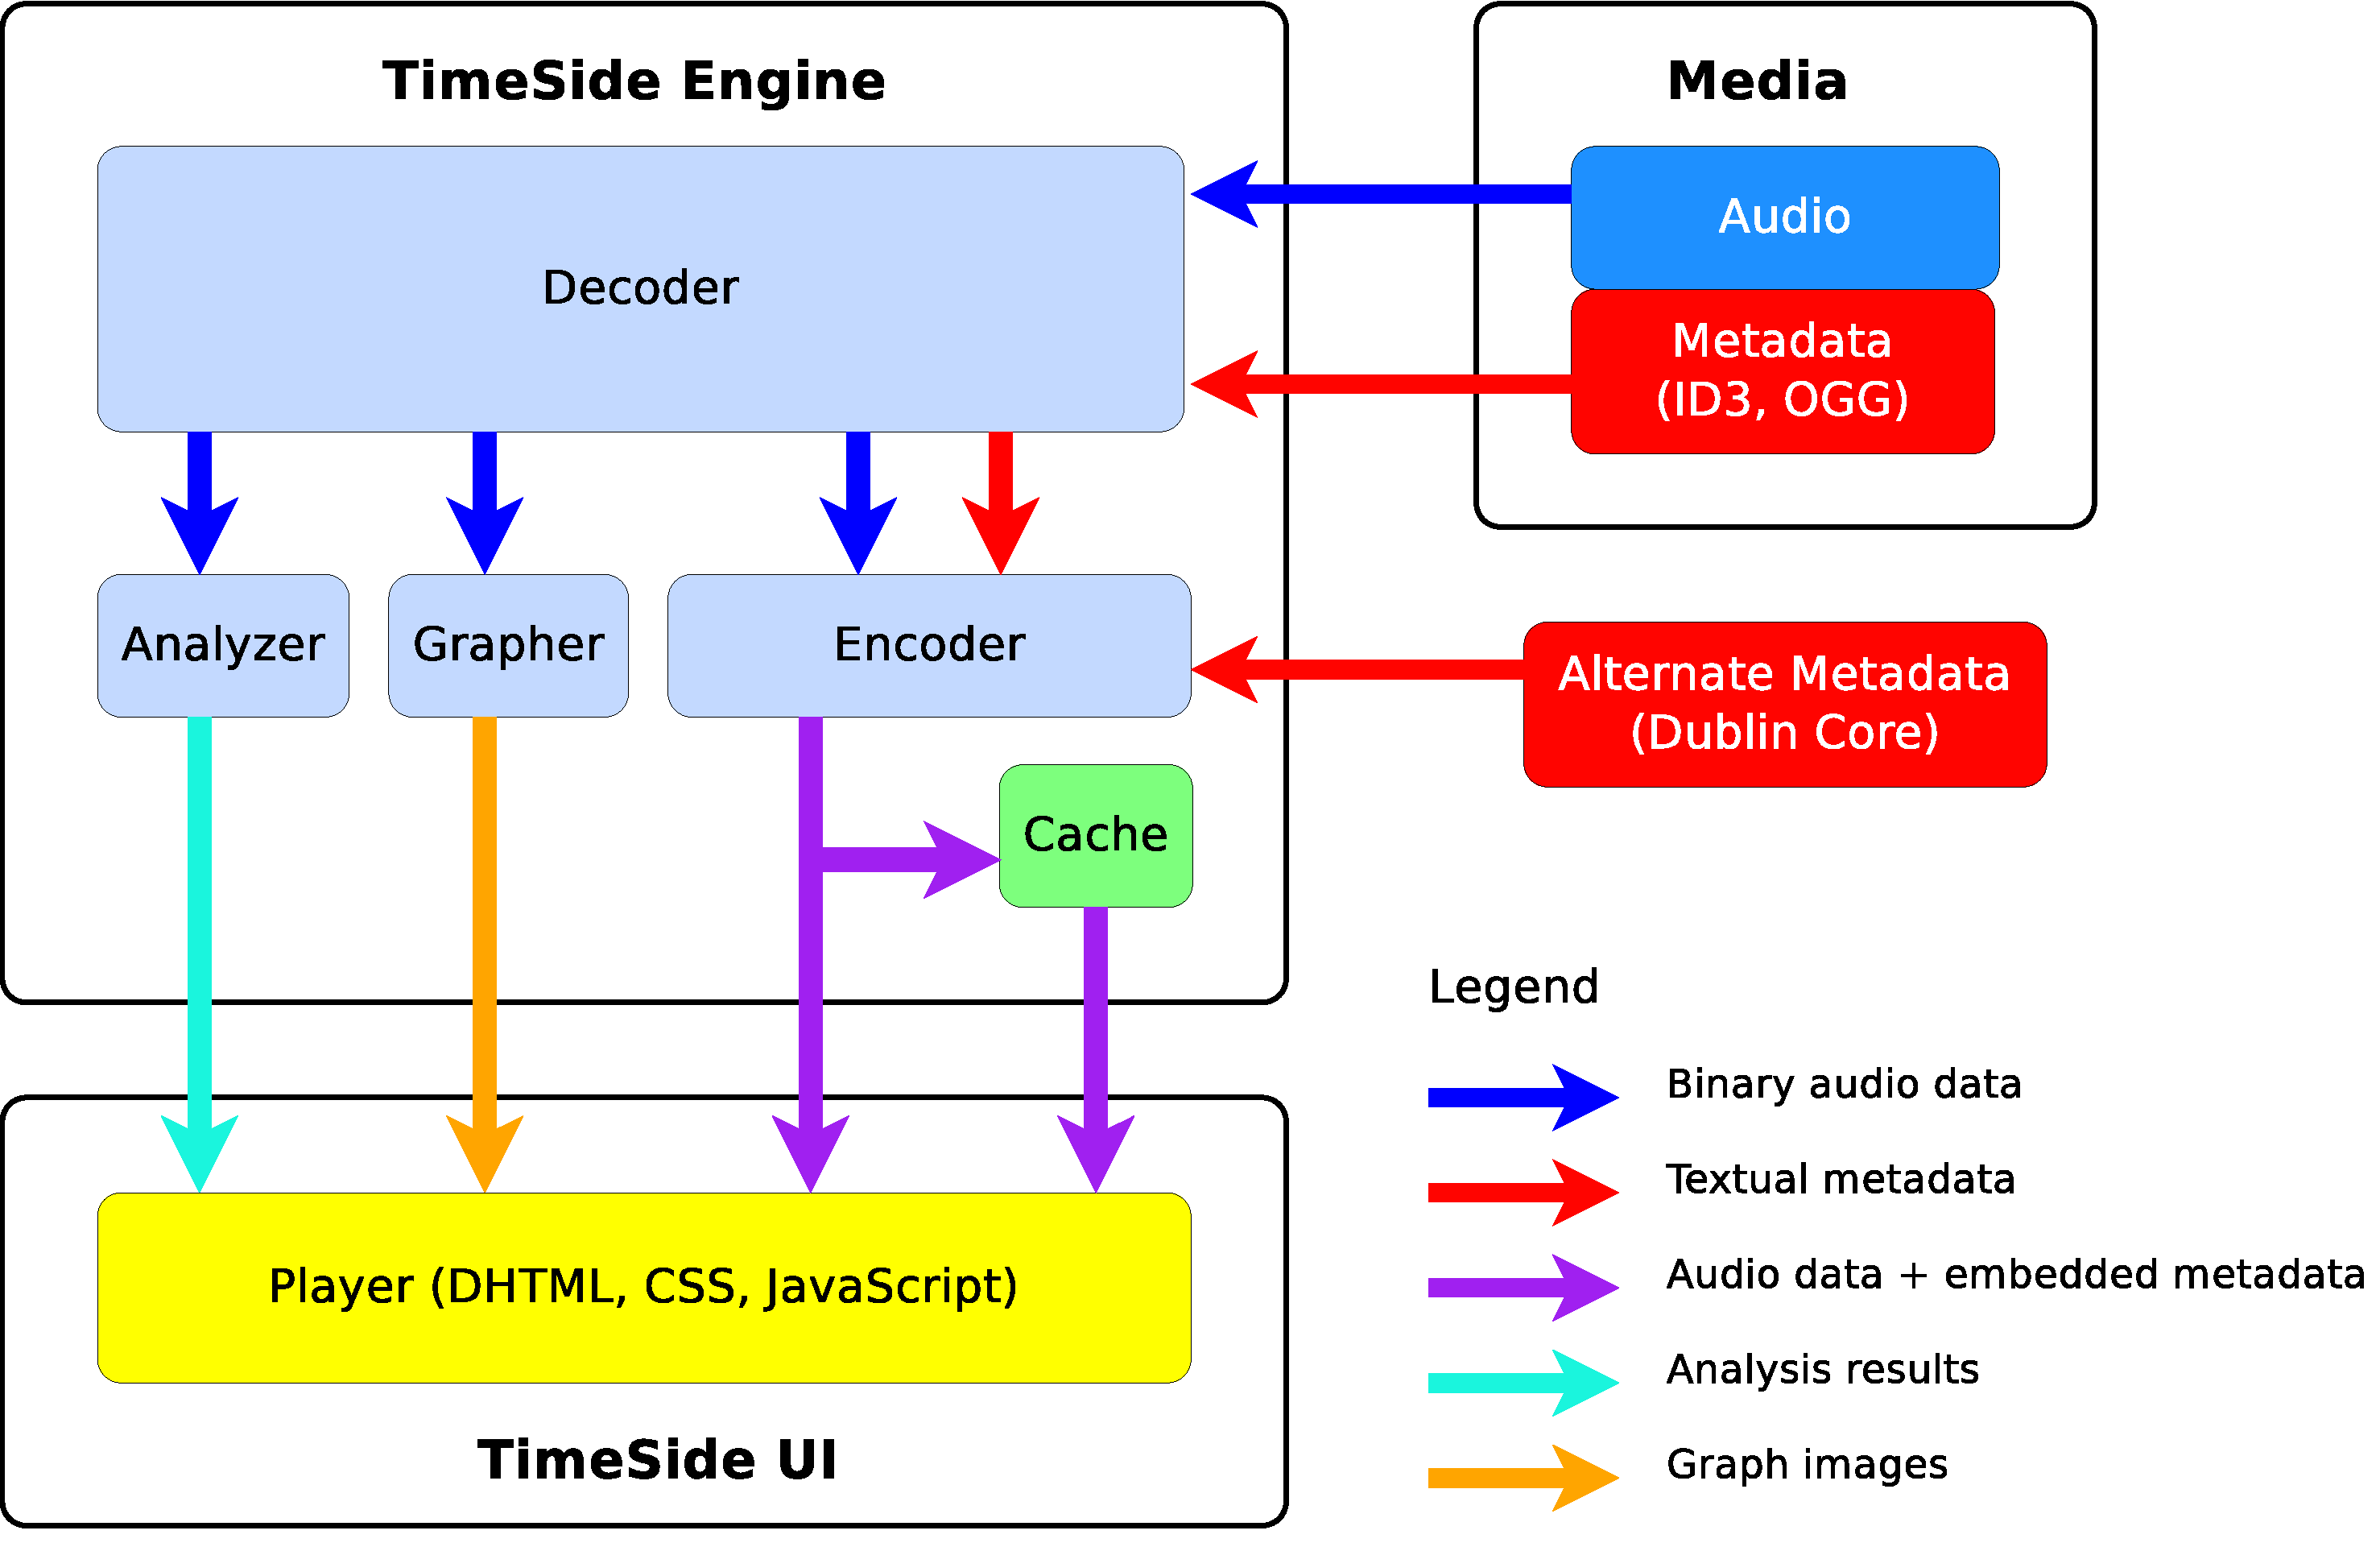
\includegraphics[width=0.4\paperwidth]{../img/timeside_schema.pdf}
  \caption{TimeSide architecture}
\end{figure}

\textbf{Goals}\\

\begin{itemize}
\item \alert{Do} asynchronous and fast audio processing with Python.
\item \alert{Decode} ANY audio or video format into numpy arrays thanks to Gstreamer.
\item \alert{Analyze} audio content with some external audio feature extraction libraries.
\item \alert{Organize}, \alert{serialize} and \alert{save} analysis metadata through various formats.
\item \alert{Draw} various fancy waveforms, spectrograms and other cool graphers.
\item \alert{Transcode} audio data in various media formats and stream them through web apps.
\item \alert{Playback}, \alert{index}, \alert{tag} and \alert{interact} on demand with a smart high-level HTML5 extensible player.
\end{itemize}

\textbf{Audio features extraction}\\
TimeSide incorporates some state-of-the-art audio feature extraction libraries such as:

  \begin{itemize}
  \item \textbf{Aubio:
      \colorbox{yellow!50}{\hskip1ex  \url{http://aubio.org} \hskip1ex }}
    \cite{brossierPhD}
  \item \textbf{Yaafe:
       \colorbox{yellow!50}{\hskip1ex \url{http://yaafe.sourceforge.net}\hskip1ex }}
    \cite{yaafe_ISMIR2010}
  \item \textbf{Vamp plugins:  
      \colorbox{yellow!50}{\hskip1ex \url{http://www.vamp-plugins.org}\hskip1ex }} 
    \cite{vamp-plugins}
    \end{itemize}


Given the extracted features, every sound item in a given collection can be automatically analyze. The results of this analysis can be displayed as a support to ethnomusicological studies.
Further works lead by the DIADEMS project will incorporate advance Music Information Retrieval methods in order to provide \alert{automatic annotation}, \alert{segmentation} and \alert{similarity} analysis.
\end{block}
\begin{block}{Code Example (Python)}
\vskip1ex
    \begin{minipage}{0.6\linewidth}
      \begin{lstlisting}

import timeside

# Define some processors:
decoder = timeside.decoder.FileDecoder('sweep.wav')
analyzer = timeside.analyzer.Level()
grapher = timeside.grapher.Spectrogram()
encoder = timeside.encoder.VorbisEncoder('sweep.ogg')

# Then, the magic pipeline:
(decoder | analyzer | grapher | encoder).run()

# Get the results:
grapher.render(output='image.png')
for key in analyzer.results.keys():
    print '%s in %s : %s'% (analyzer.results[key].name,
                            analyzer.results[key].unit,
                            analyzer.results[key].data)

\end{lstlisting}
\end{minipage}
\hskip2ex
\begin{minipage}{0.32\linewidth}
  \begin{center}
    \textbf{Results}
    \begin{figure}
      \centering
      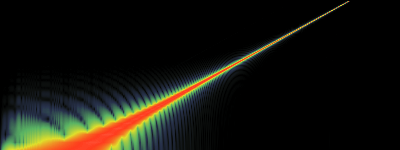
\includegraphics{img/spectrogram.png}
      \caption{Spectrogram (sweep signal)}
    \end{figure}
 \end{center} 
\vskip5ex
\begin{lstlisting}

 Level Analyzer Max:[-6.021] 
 Level Analyzer RMS:[-9.856]

\end{lstlisting}


\end{minipage}

  \end{block}
\begin{block}{Références}\tiny
\bibliographystyle{plain}
%\label{sec:ref}
\vspace{-1cm}
\begin{multicols}{2}[]
\bibliography{../aes53_Telemeta}
\end{multicols}
  \end{block}
 \end{column}
\end{columns}
\end{frame}
\end{document}
%%% Local Variables: 
%%% mode: latex
%%% TeX-master: t
%%% End: 
